%************************************************
\chapter{Esercizi Peso molecolare}\label{chp:EsercizioPM}
%************************************************
Data la distribuzione delle frazioni molecolari, tabella \ref{tab:EsercizioPM}: 
\begin{enumerate}
\item calcolare il peso molecolare medio e il peso molecolare ponderale.
\item Se il peso molecolare del monomero è $56$, calcolare il grado di polimerizzazione .
\end{enumerate}

\begin{table}
\caption{Distribuzione della media dei pesi molecolari delle frazioni polimeriche}
\label{tab:EsercizioPM}
$
\begin{array}{cc}
\toprule
M_i & \phi_i\\
\unit{\kg/\mol} & \\
\midrule
14 & 0.05\\
26 & 0.15\\
38 & 0.21\\
50 & 0.28\\
62 & 0.15\\
74 & 0.10\\
86 & 0.03\\
\bottomrule
\end{array}
$
\end{table}
Allora:
\begin{equation}
\bar{M}_n = \sum_i{\phi_iM_i} = 47.9\unit{\kg/\mol}
\end{equation}
Per calcolare la frazione ponderale a partire dalla frazione molecolare
\begin{equation}
\begin{split}
W_j &= N_j M_j\\
\frac{\psi_j}{\phi_j} &= \frac{\frac{W_j}{W}}{\frac{N_j}{N}} = \frac{\frac{W_j}{N_j}}{\frac{W}{N}}\\
&=\frac{M_j}{\bar{M}_n}
\end{split}
\end{equation}
Da cui:
\begin{equation}
\begin{split}
\psi_i &= \frac{\phi_iM_i}{\bar{M}_n}\\
\bar{M}_w &= \sum_i{\psi_iM_i} = 53.4\unit{\kg/\mol}
\end{split}
\end{equation}
Conviene calcolare \ac{IPD} per arrivare al grado di polimerizzazione:
\begin{equation}
IPD = \frac{\bar{M}_w}{\bar{M}_n} = 1.1\,\textup{monodisperso}
\end{equation}
In fine:
\begin{equation}
\begin{split}
\bar{M}_n &= \frac{W}{N} = \frac{W}{\sum_j{N_j}} = \frac{W}{\sum_j{\frac{W_j}{M_j}}} =\\
&= \frac{1}{\sum_j{\frac{W_j}{W}\frac{1}{M_j}}} = \frac{1}{\sum_j{\frac{\psi_j}{M_j}}}\\
\frac{1}{\bar{M}_n} &= \sum_j{\frac{\psi_j}{M_j}}
\end{split}
\end{equation}
\begin{equation}
\bar{n} = \frac{\bar{M}_n}{PM_{\textup{monomero}}} = \frac{53400\unit{\g/\mol}}{56\unit{\g/\mol}} = 851
\end{equation}


%************************************************
\chapter{Esercizi sulla viscoelasticità lineare}\label{chp:VisElastLineare}
%************************************************
\section{Esercizio}
$E = E(t)$ come in figura \ref{fig:Esercizio1} e storia di deformazione.
Se ne calcoli lo sforzo.

\begin{figure}
\centering
\subfloat[][\emph{Andamento rilassamento}\label{fig:Esercizio1_E}]
{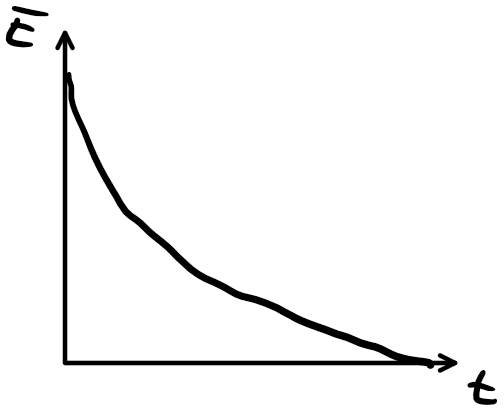
\includegraphics[width = 0.4\textwidth]{gfx/Esercizio1_E}}\quad
\subfloat[][\emph{Storia deformazione}\label{fig:Esercizio1_eps}]
{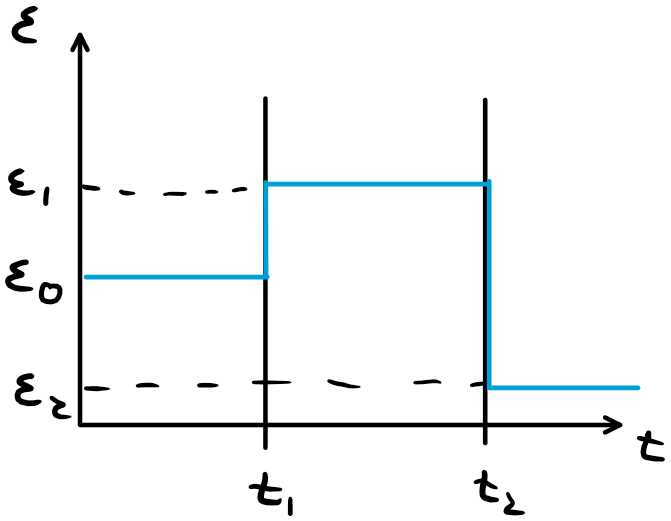
\includegraphics[width = 0.4\textwidth]{gfx/Esercizio1_eps}}
\caption{Esercizio 1 viscoelasticità lineare}
\label{fig:Esercizio1}
\end{figure}

Si nota che la funzione $\epsilon(t)$ è lineare a tratti, per cui suddivideremo in intervalli dove è lineare.
\begin{description}
\item[$0 < t < t_1$] allora:
\begin{equation}
\begin{cases}
\epsilon(t) &= \epsilon_0 \quad \forall t \in [0;t_1)\\
\sigma(t) &= \epsilon_0 E(t)
\end{cases}
\end{equation}
\item[$t_1 < t < t_2$]
In questo caso bisogna considerare che c'è il rilassamento della deformazione precedente più lo sforzo della nuova deformazione.
Da cui:
\begin{equation}
\sigma = \epsilon_0E(t) + (\epsilon_1 - \epsilon_0)E(t) = [\epsilon_0 + \epsilon_1 - \epsilon_0]E(t)???
\end{equation}
Non è corretto infatti è erronea la sovrapposizione degli effetti:
\begin{equation}
\sigma = \epsilon_0E(t) + (\epsilon_1 - \epsilon_0)E(t-t_1)
\end{equation}
\item[$t>t_2$] per lo stesso ragionamento precedente:
\begin{equation}
\sigma = \epsilon_0E(t) + (\epsilon_1 - \epsilon_0)E(t-t_1) + (\epsilon_2 - \epsilon_1)E(t - t_2)
\end{equation}
\end{description}

\begin{figure}
\centering
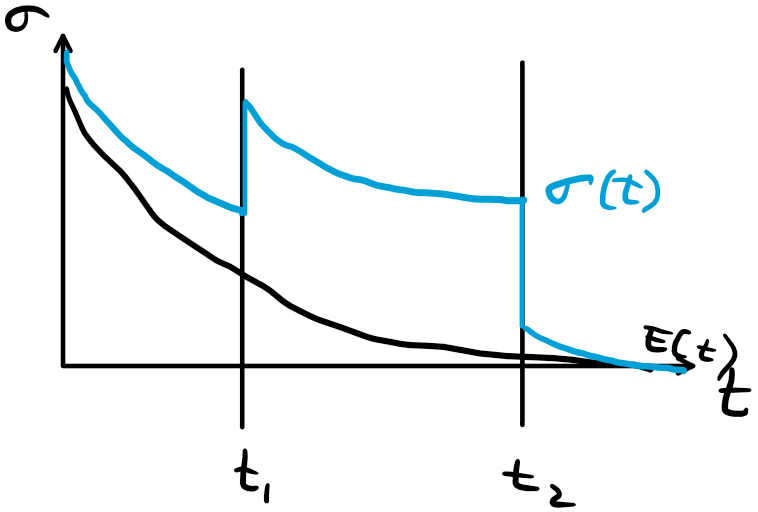
\includegraphics[width = \textwidth]{gfx/Risultato1}
\caption{Risultato dell'esercizio 1}
\label{fig:Risultato1}
\end{figure}

\section{Esercizio}
Confronto di due storie di deformazione differenti:

\begin{figure}
\centering
\subfloat[][\emph{Andamento rilassamento}\label{fig:Esercizio2_E}]
{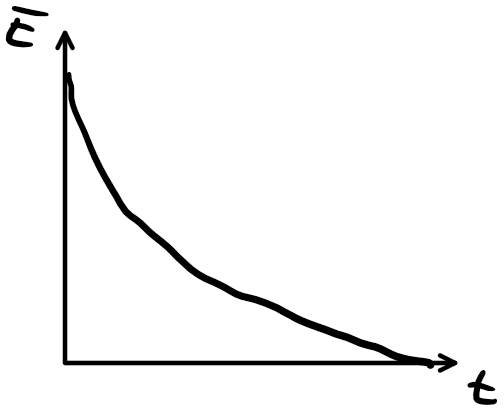
\includegraphics[width = 0.4\textwidth]{gfx/Esercizio1_E}}\quad
\subfloat[][\emph{Storie di deformazione}\label{fig:Esercizio2_eps}]
{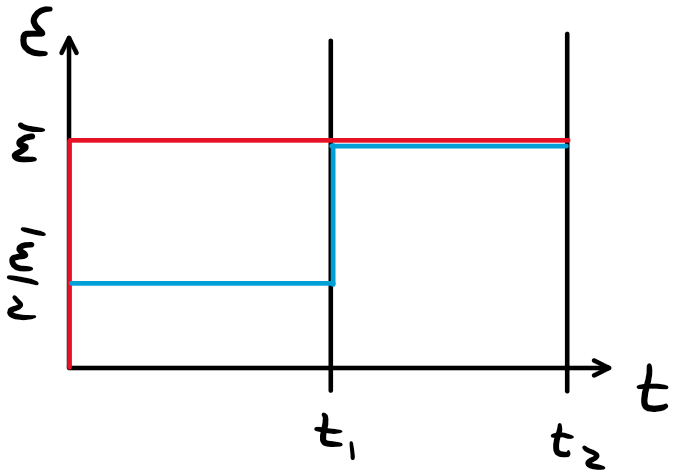
\includegraphics[width = 0.4\textwidth]{gfx/Esercizio2_eps}}
\caption{Andamenti per il confronto delle due storie di deformazione}
\label{fig:Esercizio2}
\end{figure}

\paragraph{Soluzione}
allora:
\begin{description}
\item[Storia rossa \ref{fig:Esercizio2_eps}] $\epsilon = \bar{\epsilon} \Rightarrow \sigma(t_2) = \bar{\epsilon}E(t_2)$
\item[Storia azzurra \ref{fig:Esercizio2_eps}] in questo caso:
\begin{equation}
\sigma(t_2) =%
\begin{cases}
\frac{\bar{\epsilon}}{2} &0<t<t_1\\
\bar{\epsilon} &t_1<t<t_2
\end{cases}
\end{equation}
\end{description}
Ne caso della seconda storia, osserviamo l'andamento dello sforzo:
\begin{equation}
\sigma(t_2) = \frac{\bar{\epsilon}}{2}E(t_2) + [\bar{\epsilon} - \frac{\bar{\epsilon}}{2}]E(t_2 - t_1)
\end{equation}
Ne risulta che siccome $t_2 > t_2-t_1$ e siccome la deformazione è una funzione decrescente: $E(t_2)< E(t_2-t_1)$.
Dunque lo sforzo conseguente la storia rossa è minore di quella azzurra.

\section{Esercizio}
Considerando un solido a tre parametri come in figura \ref{fig:Esercizio3_Fluido}.
Con le differenti storie di deformazione \ref{fig:Esercizio3_eps1} e \ref{fig:Esercizio3_eps2}.

\begin{figure}
\centering
\subfloat[][\emph{Solido a tre parametri}\label{fig:Esercizio3_Fluido}]
{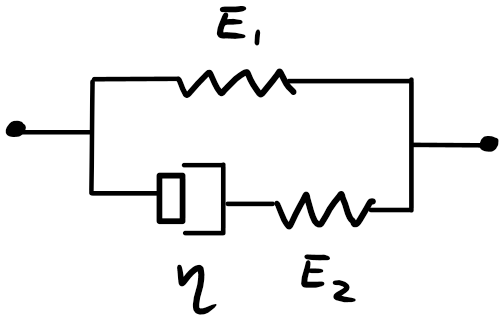
\includegraphics[width = 0.5\textwidth]{gfx/Esercizio3_Fluido}}\\
\subfloat[][\emph{Prima storia di deformazione}\label{fig:Esercizio3_eps1}]
{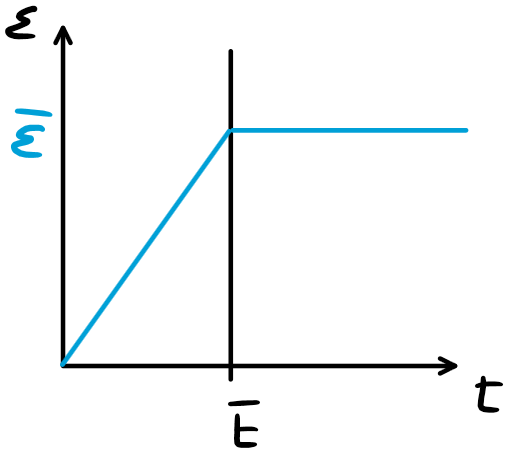
\includegraphics[width = 0.4\textwidth]{gfx/Esercizio3_eps1}}\quad
\subfloat[][\emph{Seconda storia di deformazione}\label{fig:Esercizio3_eps2}]
{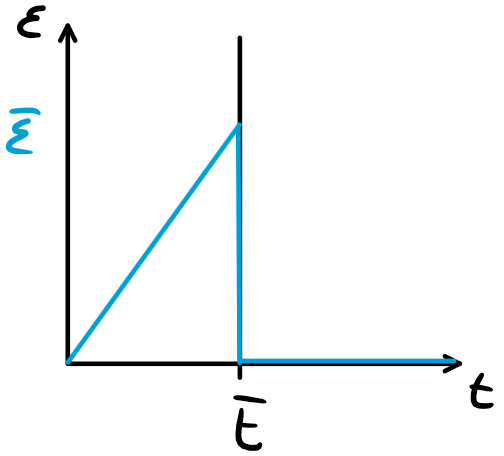
\includegraphics[width = 0.4\textwidth]{gfx/Esercizio3_eps2}}
\caption{Esercizio 3}
\label{fig:Esercizio3}
\end{figure}

\paragraph{Soluzione}
Allora:
\begin{equation}
\begin{split}
\dot{\epsilon} &= \dot{\epsilon}_1 + \dot{\epsilon}_3 = \frac{\dot{\sigma}_2}{E_2} + \frac{\dot{\sigma}_3}{\eta_3}\\
&=\frac{\dot{\sigma}}{E_2} - \frac{\dot{\sigma}_1}{E_2} + \frac{\sigma}{\eta_3} - \frac{\sigma_1}{\eta_3}\\
&= \frac{\dot{\sigma}}{E_2} - \frac{E_1\dot{\epsilon}}{E_2} + \frac{\sigma}{\eta_3} - \frac{\sigma_1\epsilon}{\eta_3}\\
\frac{\dot{\sigma}}{E_2} &+\frac{\sigma}{\eta_3} = \left(1 + \frac{E_1}{E_2}\right)\dot{\epsilon} + \frac{E_1}{\eta_3}\epsilon
\end{split}
\end{equation}

Imponiamo la storia di deformazione \ref{fig:Esercizio3_eps1}:
\begin{equation}
\epsilon(t) = \frac{\bar{\epsilon}}{\bar{t}}t \qquad \dot{\epsilon} = \frac{\bar{\epsilon}}{\bar{t}}
\end{equation}
Applicandolo, all'equazione differenziale:
\begin{equation}
\begin{split}
\frac{\dot{\sigma}}{E_2}&+\frac{\sigma}{\eta_3} = \left(1+\frac{E_1}{E_2}\right)\frac{\bar{\epsilon}}{\bar{t}} + \frac{E_1}{\eta_3}\frac{\bar{\epsilon}}{\bar{t}}t\\
\sigma(t) &= \sigma_h + \sigma_p =%
\begin{cases}
\sigma_h(t) = C e^{-\frac{t}{\tau_r}} \quad \tau_r = \frac{\eta_3}{E_2}\\
\sigma_p(t) = A+Bt
\end{cases}
\end{split}
\end{equation}
Affinché sia soluzione deve valere che l'equazione abbia soluzione nelle componenti omogenee e particolare.
Dunque sostituiamo a $\sigma$, $\sigma_p$.
\begin{equation}
\begin{split}
\frac{B}{E_2} &+ \frac{A}{\eta_3} + \frac{B}{\eta_3}t = \left(1+\frac{E_1}{E_2}\right)\frac{\bar{\epsilon}}{\bar{t}} + \frac{E_1}{\eta_3}\frac{\bar{\epsilon}}{\bar{t}}t\\
&\begin{cases}
B = E_1\frac{\bar{\epsilon}}{\bar{t}}\\
A = \eta_3 \frac{\epsilon}{\bar{t}}
\end{cases}\\
\sigma(t) &= \eta_3 \frac{\bar{\epsilon}}{\bar{t}} + E_1\frac{\bar{\epsilon}}{\bar{t}}t + C e^{-\frac{t}{\tau_r}}\\
t &= 0 \rightarrow 0 = \eta_3 \frac{\bar{\epsilon}}{\bar{t}} + C \Rightarrow C = -\eta_3\frac{\bar{\epsilon}}{\bar{t}}\\
\sigma(t) &= E_1\frac{\bar{\epsilon}}{\bar{t}}t + \eta_3\frac{\bar{\epsilon}}{\bar{t}}\left(1 - e^{-\frac{t}{\tau_r}}\right) 
\end{split}
\end{equation}

Il secondo tratto della storia di deformazione è costante, per cui vale:
\begin{equation}
\frac{\dot{\sigma}}{E_2} + \frac{\sigma}{\eta_3} = \frac{E_1}{\eta_3}\bar{\epsilon}
\end{equation}
Allora:
\begin{equation}
\sigma(t) = C e^{-\frac{t}{\tau_r}} + E_1\bar{\epsilon}
\end{equation}
In $t = \bar{t}$:
\begin{equation}
\begin{split}
\sigma(t) &= E_1\bar{\epsilon} + \eta_3\frac{\bar{\epsilon}}{\bar{t}}\left(1 - e^{-\frac{\bar{t}}{\tau_r}}\right)\\
\sigma(t) &= E_1\bar{\epsilon} + \eta_3\frac{\bar{\epsilon}}{\bar{t}}\left(e^{-\frac{t-\bar{t}}{\tau_r}} - e^{-\frac{t}{\tau_r}}\right)
\end{split}
\end{equation}
La soluzione dovrebbe essere quella in figura \ref{fig:Soluzione3}.
Per la storia di deformazione \ref{fig:Esercizio3_eps2}
la soluzione sta nel considerare la discontinuità come $-(E_1 - E_2)\bar{\epsilon}$

\begin{figure}
\centering
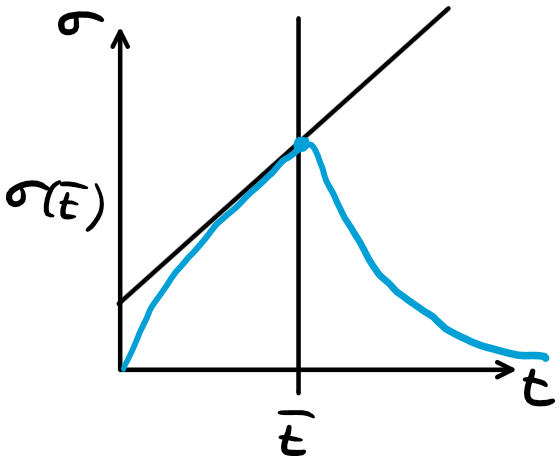
\includegraphics[width = 0.5\textwidth]{gfx/Soluzione3}
\caption{Soluzione dell'esercizio}
\label{fig:Soluzione3}
\end{figure}
%************************************************
\chapter{Tavola periodica}\label{chp:Tavolaperiodica}
%************************************************
\newpage
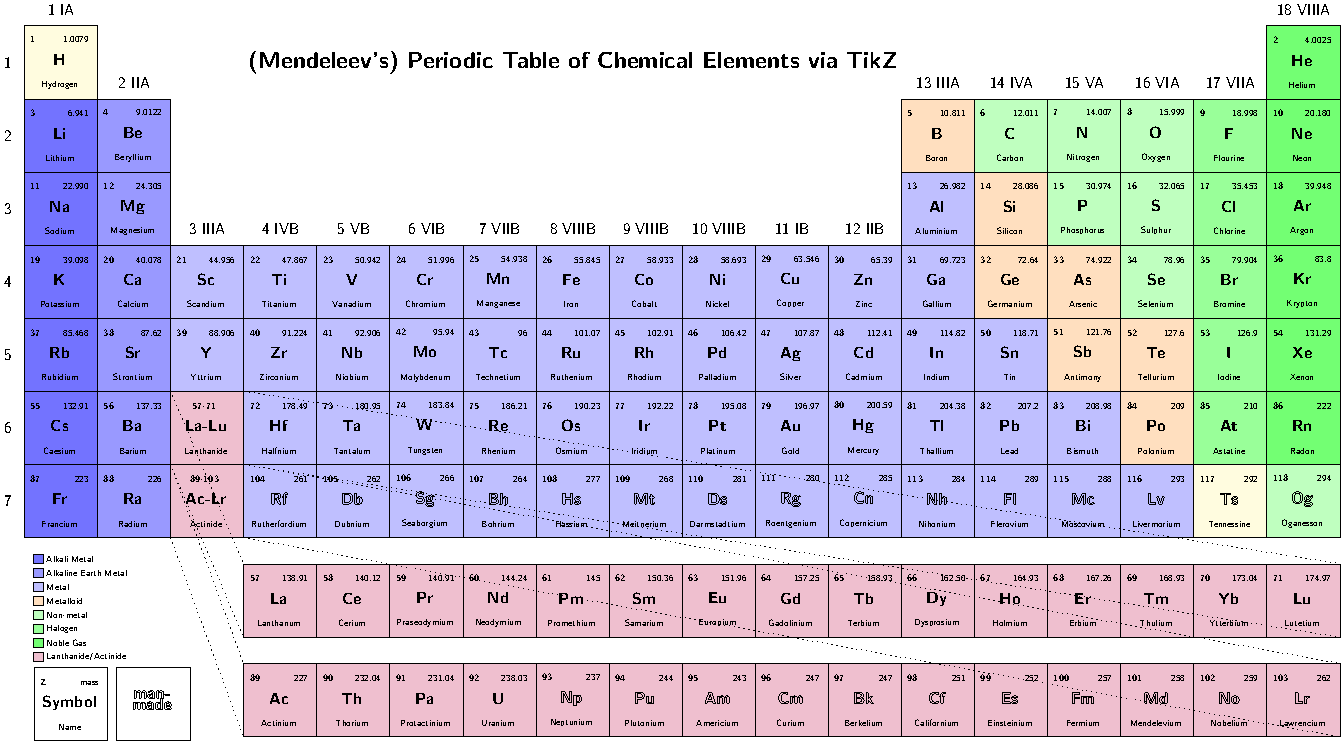
\includegraphics[scale = 1, angle = 90]{gfx/Periodic_table2017}